% !TeX root = cpp-esc22.tex

\usetikzlibrary{positioning}
\newlength{\bytesize}
\newlength{\memwidth}
\newlength{\memheight}

\section{Containers}

\begin{frame}[fragile]{Dynamic memory allocation}

  It's not always possible to know at compile time which type of objects is
  needed or how many of them
  \begin{itemize}

  \item<2-> run-time polymorphism
    \begin{codeblock}
struct Shape \{ \ddd \};
struct Rectangle : Shape \{ \ddd \};
struct Circle : Shape \{ \ddd \};

std::unique_ptr<Shape> s;
char c; std::cin >{}> c;
switch (c) \{
 case \upquote{r}: s = std::make_unique<Rectangle>(); break;
 case \upquote{c}: s = std::make_unique<Circle>(); break;
\}\end{codeblock}

  \item<3-> dynamic collections of objects
    \begin{codeblock}
int n; std::cin >{}> n;
std::vector<Particle> v;
for (int i = 0; i != n; ++i) \{
  v.emplace_back(\ddd);
\}\end{codeblock}

  \end{itemize}
\end{frame}

\begin{frame}[fragile]{Stack vs Heap: space}

  \begin{columns}[T]
    \begin{column}{.3\textwidth}

  \begin{codeblock}{
struct S \{
  int    n;
  float  f;
  double d;
\};

\uncover<2->{auto foo_s() \{
  S s;
  \ddd
\}}

\uncover<4->{auto foo_h() \{
  S* s = new S;
  \ddd
\}}}\end{codeblock}
    \end{column}

    \setlength{\bytesize}{0.2cm}
    \setlength{\memwidth}{8\bytesize}
    \setlength{\memheight}{5cm}

    \begin{column}{.3\textwidth}
      \uncover<2->{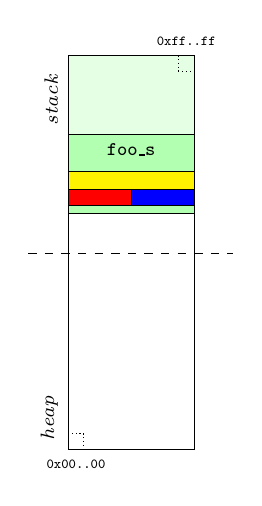
\begin{tikzpicture}
        [anchor=south west]
        \node (memory) at (0,0) [
          rectangle,
          minimum width=\memwidth,
          minimum height=\memheight,
          draw=black
        ] {};
        \node at (0,3) [
          rectangle,
          minimum width=\memwidth,
          minimum height=5\bytesize,
          draw=black,
          fill=green!30!white,
          label={[yshift=-.4cm]\scriptsize\tt foo\_s}
        ] {};
        \node at (0,4) [
          rectangle,
          minimum width=\memwidth,
          minimum height=1cm,
          draw=black,
          fill=green!10!white
        ] {};
        \node at (0,3.1) [
          rectangle,
          minimum width=.5\memwidth,
          minimum height=\bytesize,
          draw=black,
          fill=red
        ] {};
        \node at (.5\memwidth,3.1) [
          rectangle,
          minimum width=.5\memwidth,
          minimum height=\bytesize,
          draw=black,
          fill=blue
        ] {};
        \node at (0,3.1cm + \bytesize) [
          rectangle,
          minimum width=\memwidth,
          minimum height=\bytesize,
          draw=black,
          fill=yellow
        ] {};
        \node at (0,0) [
          rectangle,
          inner sep=0pt,
          minimum width=\bytesize,
          minimum height=\bytesize,
          draw=black,
          densely dotted,
          label={270:{\tiny\tt 0x00..00}}
        ] {};
        \node at (\memwidth-\bytesize,\memheight-\bytesize) [
          rectangle,
          inner sep=0pt,
          minimum width=\bytesize,
          minimum height=\bytesize,
          draw=black,
          densely dotted,
          label={90:{\tiny\tt 0xff..ff}}
        ] {};
        \draw [dashed] (-.5cm,.5\memheight) -- (\memwidth + .5cm,.5\memheight);
        \node at (0,4) [rotate=90] {\scriptsize\textit{stack}};
        \node at (0,0) [rotate=90] {\scriptsize\textit{heap}};
      \end{tikzpicture}}

      \uncover<3->{\scriptsize Occupancy:
      \begin{itemize}
      \item \code{sizeof(S)}
      \end{itemize}}

    \end{column}

    \begin{column}{.3\textwidth}

      \uncover<4->{\begin{tikzpicture}
        [anchor=south west]
        \node (memory) at (0,0) [
          rectangle,
          minimum width=\memwidth,
          minimum height=\memheight,
          draw=black
        ] {};
        \node at (0,3) [
          rectangle,
          minimum width=\memwidth,
          minimum height=5\bytesize,
          draw=black,
          fill=green!30!white,
          label={[yshift=-.4cm]\scriptsize\tt foo\_h}
        ] {};
        \node at (0,4) [
          rectangle,
          minimum width=\memwidth,
          minimum height=1cm,
          draw=black,
          fill=green!10!white
        ] {};
        \node (ptr) at (0,3.1cm) [
          rectangle,
          minimum width=\memwidth,
          minimum height=\bytesize,
          draw=black,
          fill=green
        ] {};
        \node at (0,1.1) [
          rectangle,
          minimum width=.5\memwidth,
          minimum height=\bytesize,
          draw=black,
          fill=red
        ] {};
        \node at (.5\memwidth,1.1) [
          rectangle,
          minimum width=.5\memwidth,
          minimum height=\bytesize,
          draw=black,
          fill=blue
        ] {};
        \node (alloc) at (0,1.1cm + \bytesize) [
          rectangle,
          minimum width=\memwidth,
          minimum height=\bytesize,
          draw=black,
          fill=yellow
        ] {};
        \draw[Circle-Stealth,black!80] (ptr.east) .. controls +(.5,-1) .. (alloc.north east);
        \node at (0,0) [
          rectangle,
          inner sep=0pt,
          minimum width=\bytesize,
          minimum height=\bytesize,
          draw=black,
          densely dotted,
          label={270:{\tiny\tt 0x00..00}}
        ] {};
        \node at (\memwidth-\bytesize,\memheight-\bytesize) [
          rectangle,
          inner sep=0pt,
          minimum width=\bytesize,
          minimum height=\bytesize,
          draw=black,
          densely dotted,
          label={90:{\tiny\tt 0xff..ff}}
        ] {};
        \draw [dashed] (-.5cm,.5\memheight) -- (\memwidth + .5cm,.5\memheight);
        \node at (0,4) [rotate=90] {\scriptsize\textit{stack}};
        \node at (0,0) [rotate=90] {\scriptsize\textit{heap}};
      \end{tikzpicture}}

      \uncover<5->{\scriptsize Occupancy:
      \begin{itemize}
      \item \code{sizeof(S)} + \code{sizeof(S*)}
      \item plus \code{new} internal space overhead
      \end{itemize}}

    \end{column}
  \end{columns}
\end{frame}

\begin{frame}[fragile]{Stack vs Heap: time}
  \begin{columns}[T]
    \begin{column}{.4\textwidth}
      Stack
      \begin{codeblock}{\tiny
void stack()
\{
  int m\{123\};
  \ddd
\}}\end{codeblock}
      \begin{codeblock}<2->{\tiny
stack():
     subq %4, %rsp
     movl $123, (%rsp)
     \ddd
     addq $4, %rsp
     ret}\end{codeblock}
    \end{column}

    \begin{column}{.6\textwidth}
      Heap
      \begin{codeblock}{\tiny
void heap()
\{
  int* m = new int\{123\};
  \ddd
  delete m;
\}}\end{codeblock}
      \begin{codeblock}<3->{\tiny
heap():
     subq	$8, %rsp
     movl	$4, %edi
     call	operator new(unsigned long)
     movl	$123, (%rax)
     movq %rax, (%rsp)
     \ddd
     movl	$4, %esi
     movq	%rax, %rdi
     call	operator delete(void*, unsigned long)
     addq	$8, %rsp
     ret}\end{codeblock}
      \begin{codeblock}<4->{\tiny
$ g++ -O3 heap.cpp && ./a.out
1000000 heap() calls in 0.0205281 s}\end{codeblock}

\uncover<4->{\scriptsize i.e. \~20 ns just to allocate/deallocate an \code{int}}

    \end{column}
  \end{columns}
\end{frame}

\begin{frame}[fragile]{Google Benchmark}

  \begin{itemize}
  \item \url{https://github.com/google/benchmark}
    \begin{codeblock}
static void BM_Stack(benchmark::State& state) \{
  while (state.KeepRunning()) \{
    int m\{123\};
  \}
\}
BENCHMARK(BM_Stack);

static void BM_Heap(benchmark::State& state) \{
  while (state.KeepRunning()) \{
    auto m = std::make_unique<int>(123);
  \}
\}
BENCHMARK(BM_Heap);
  \end{codeblock}

  \item Hands-on
    \begin{itemize}
    \item start from {\footnotesize\url{https://quick-bench.com/q/GU6FHQwPuvX-JV4ITLIW00my71Y}}
      \begin{itemize}
      \item note the use of \code{benchmark::DoNotOptimize()}
      \end{itemize}
    \item play with the optimization level and the code
    \end{itemize}

  \end{itemize}

\end{frame}

\begin{frame}{STL Containers}

  \begin{itemize}
  \item Objects that contain and own other objects
  \item Different characteristics and operations, some common traits
  \item Implemented as class templates
  \end{itemize}

  \begin{description}
  \item[Sequence] The client decides where an element gets inserted
    \begin{itemize}
    \item \code{array}, \code{deque}, \code{forward\_list}, \code{list}, \code{vector}
    \end{itemize}
  \item[Associative] The container decides where an element gets
    inserted
    \begin{description}
    \item[Ordered] The elements are sorted
      \begin{itemize}
      \item \code{map}, \code{multimap}, \code{set}, \code{multiset}
      \end{itemize}
    \item[Unordered] The elements are hashed
      \begin{itemize}
      \item \code{unordered\_*}
      \end{itemize}
    \end{description}
  \end{description}

\end{frame}

\begin{frame}[fragile]{Sequence containers}

  \setlength{\bytesize}{0.2cm}
  \setlength{\memwidth}{8\bytesize}
  \setlength{\memheight}{5cm}

  \begin{columns}[T]
    \begin{column}{.3\textwidth}

      \code{std::array}

      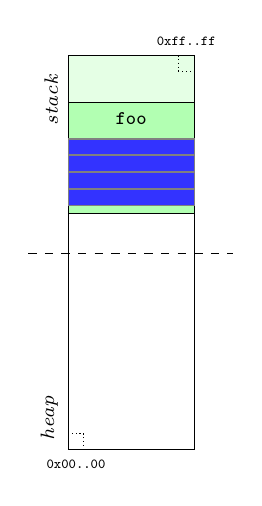
\begin{tikzpicture}[
          word/.style={
            draw=black!50,
            minimum height=\bytesize,
            minimum width=8\bytesize,
            fill=blue!80!white,
            inner sep=0pt
          },
          anchor=south west
        ]
        \node (memory) at (0,0) [
          rectangle,
          minimum width=\memwidth,
          minimum height=\memheight,
          draw=black
        ] {};
        \node at (0,.7\memheight) [
          rectangle,
          minimum width=\memwidth,
          minimum height=.3\memheight,
          draw=black,
          fill=green!10!white
        ] {};
        \node at (0,.5\memheight+.5cm) [
          rectangle,
          minimum width=\memwidth,
          minimum height=7\bytesize,
          draw=black,
          fill=green!30!white,
          label={[yshift=-0.4cm]\scriptsize\tt foo}
        ] {};
        \node (word1) at (0,3.1cm) [word] {};
        \node (word2) [word,above=0 of word1] {};
        \node (word3) [word,above=0 of word2] {};
        \node (word4) [word,above=0 of word3] {};
        \node at (0,0) [
          rectangle,
          inner sep=0pt,
          minimum width=\bytesize,
          minimum height=\bytesize,
          draw=black,
          densely dotted,
          label={270:{\tiny\tt 0x00..00}}
        ] {};
        \node at (\memwidth-\bytesize,\memheight-\bytesize) [
          rectangle,
          inner sep=0pt,
          minimum width=\bytesize,
          minimum height=\bytesize,
          draw=black,
          densely dotted,
          label={90:{\tiny\tt 0xff..ff}}
        ] {};
        \draw [dashed] (-.5cm,.5\memheight) -- (\memwidth + .5cm,.5\memheight);
        \node at (0,4) [rotate=90] {\scriptsize\textit{stack}};
        \node at (0,0) [rotate=90] {\scriptsize\textit{heap}};
      \end{tikzpicture}
    \end{column}

    \begin{column}{.3\textwidth}<2->

      \code{std::vector}

      \begin{tikzpicture}[
          word/.style={
            draw=black!50,
            minimum height=\bytesize,
            minimum width=8\bytesize,
            fill=blue!80!white,
            inner sep=0pt
          },
          anchor=south west
        ]
        \node (memory) at (0,0) [
          rectangle,
          minimum width=\memwidth,
          minimum height=\memheight,
          draw=black
        ] {};
        \node at (0,.7\memheight) [
          rectangle,
          minimum width=\memwidth,
          minimum height=.3\memheight,
          draw=black,
          fill=green!10!white
        ] {};
        \node at (0,.5\memheight+.5cm) [
          rectangle,
          minimum width=\memwidth,
          minimum height=6\bytesize,
          draw=black,
          fill=green!30!white,
          label={[yshift=-0.4cm]\scriptsize\tt foo}
        ] {};
        \node (beg) at (0,3.1cm) [word,green!50!black,draw=black!50!white] {};
        \node (end) [word,above=0 of beg,green!50!black,draw=black!50!white] {};
        \node (cap) [word,above=0 of end,green!50!black,draw=black!50!white] {};
        \node (word1) at (0,.4cm) [word] {};
        \node (word2) [word,above=0 of word1] {};
        \node (word3) [word,above=0 of word2] {};
        \node (word4) [word,above=0 of word3] {};
        \node (word5) [word,above=0 of word4,blue!20!white,draw=black!50!white] {};
        \node (word6) [word,above=0 of word5,blue!20!white,draw=black!50!white] {};
        \node (word7) [word,above=0 of word6,blue!20!white,draw=black!50!white] {};
        \node (word8) [word,above=0 of word7,blue!20!white,draw=black!50!white] {};
        \node (sentinel) [word,draw=none,fill=none,above=0 of word8] {};
        \draw[{Circle[length=2pt]}-Stealth,black!80] (beg.east) .. controls +(.5,-2) .. (word1.east);
        \draw[{Circle[length=2pt]}-Stealth,black!80] (end.east) .. controls +(.5,-1.5) .. (word5.east);
        \draw[{Circle[length=2pt]}-Stealth,black!80] (cap.east) .. controls +(.5,-1) .. (sentinel.east);
        \node at (0,0) [
          rectangle,
          inner sep=0pt,
          minimum width=\bytesize,
          minimum height=\bytesize,
          draw=black,
          densely dotted,
          label={270:{\tiny\tt 0x00..00}}
        ] {};
        \node at (\memwidth-\bytesize,\memheight-\bytesize) [
          rectangle,
          inner sep=0pt,
          minimum width=\bytesize,
          minimum height=\bytesize,
          draw=black,
          densely dotted,
          label={90:{\tiny\tt 0xff..ff}}
        ] {};
        \draw [dashed] (-.5cm,.5\memheight) -- (\memwidth + .5cm,.5\memheight);
        \node at (0,4) [rotate=90] {\scriptsize\textit{stack}};
        \node at (0,0) [rotate=90] {\scriptsize\textit{heap}};
      \end{tikzpicture}
    \end{column}

    \begin{column}{.3\textwidth}<3->

      \code{std::list}

      \begin{tikzpicture}[
          word/.style={
            draw=black!50,
            minimum height=\bytesize,
            minimum width=8\bytesize,
            fill=blue!80!white,
            inner sep=0pt
          },
          anchor=south west
        ]
        \node (memory) at (0,0) [
          rectangle,
          minimum width=\memwidth,
          minimum height=\memheight,
          draw=black
        ] {};
        \node at (0,.7\memheight) [
          rectangle,
          minimum width=\memwidth,
          minimum height=.3\memheight,
          draw=black,
          fill=green!10!white
        ] {};
        \node at (0,.5\memheight+.5cm) [
          rectangle,
          minimum width=\memwidth,
          minimum height=6\bytesize,
          draw=black,
          fill=green!30!white,
          label={[yshift=-0.4cm]\scriptsize\tt foo}
        ] {};
        \node (beg) at (0,3.1cm) [word,green!50!black,draw=black!50!white] {};
        \node (end) [word,above=0 of beg,green!50!black,draw=black!50!white] {};
        \node (size) [word,above=0 of end,green!60!black,draw=black!50!white] {};
        \node (word1) at (0,1.8cm) [word] {};
        \node (next1) [word,above=0 of word1,red!70!white,draw=black!50!white] {};
        \node (prev1) [word,above=0 of next1,yellow!80!black,draw=black!50!white] {};
        \node (word2) at (0,.2cm) [word] {};
        \node (next2) [word,above=0 of word2,red!70!white,draw=black!50!white] {};
        \node (prev2) [word,above=0 of next2,yellow!80!black,draw=black!50!white] {};
        \node (word3) at (0,1.cm) [word] {};
        \node (next3) [word,above=0 of word3,red!70!white,draw=black!50!white] {};
        \node (prev3) [word,above=0 of next3,yellow!80!black,draw=black!50!white] {};
        \draw[{Circle[length=2pt]}-Stealth,black!80] (beg.east) .. controls +(.5,-.5) .. (word1.east);
        \draw[{Circle[length=2pt]}-Stealth,black!80] (end.west) .. controls +(-.5,-1.5) .. (word3.west);
        \draw[{Circle[length=2pt]}-Stealth,black!80] (next1.east) .. controls +(.5,-.4) .. (word2.east);
        \draw[{Circle[length=2pt]}-Stealth,black!80] (next2.west) .. controls +(-.5,.3) .. (word3.west);
        \draw[{Circle[length=2pt]}-Stealth,black!80] (prev2.east) .. controls +(.3,1) .. (word1.east);
        \draw[{Circle[length=2pt]}-Stealth,black!80] (prev3.west) .. controls +(-.5,-1) .. (word2.west);
        \draw[{Circle[length=2pt]}-{Rectangle[length=2pt,width=5pt]},black!80] (prev1.east) -- +(.5,0);
        \draw[{Circle[length=2pt]}-{Rectangle[length=2pt,width=5pt]},black!80] (next3.west) -- +(-.5,0);
        \node at (0,0) [
          rectangle,
          inner sep=0pt,
          minimum width=\bytesize,
          minimum height=\bytesize,
          draw=black,
          densely dotted,
          label={270:{\tiny\tt 0x00..00}}
        ] {};
        \node at (\memwidth-\bytesize,\memheight-\bytesize) [
          rectangle,
          inner sep=0pt,
          minimum width=\bytesize,
          minimum height=\bytesize,
          draw=black,
          densely dotted,
          label={90:{\tiny\tt 0xff..ff}}
        ] {};
        \draw [dashed] (-.5cm,.5\memheight) -- (\memwidth + .5cm,.5\memheight);
        \node at (0,4) [rotate=90] {\scriptsize\textit{stack}};
        \node at (0,0) [rotate=90] {\scriptsize\textit{heap}};
      \end{tikzpicture}
    \end{column}
  \end{columns}
\end{frame}

\begin{frame}[fragile]{Associative ordered containers}

  \begin{itemize}
  \item They contain ordered values (\code{set} and \code{multiset}) or
    key-value pairs (\code{map} and \code{multimap})
  \item Search, removal and insertion have logarithmic complexity
  \item<2-> Typically implemented as balanced (red-black) trees
  \end{itemize}

  \begin{columns}
    \begin{column}{.5\textwidth}<2->
      \tikz \node (rbtree)
            {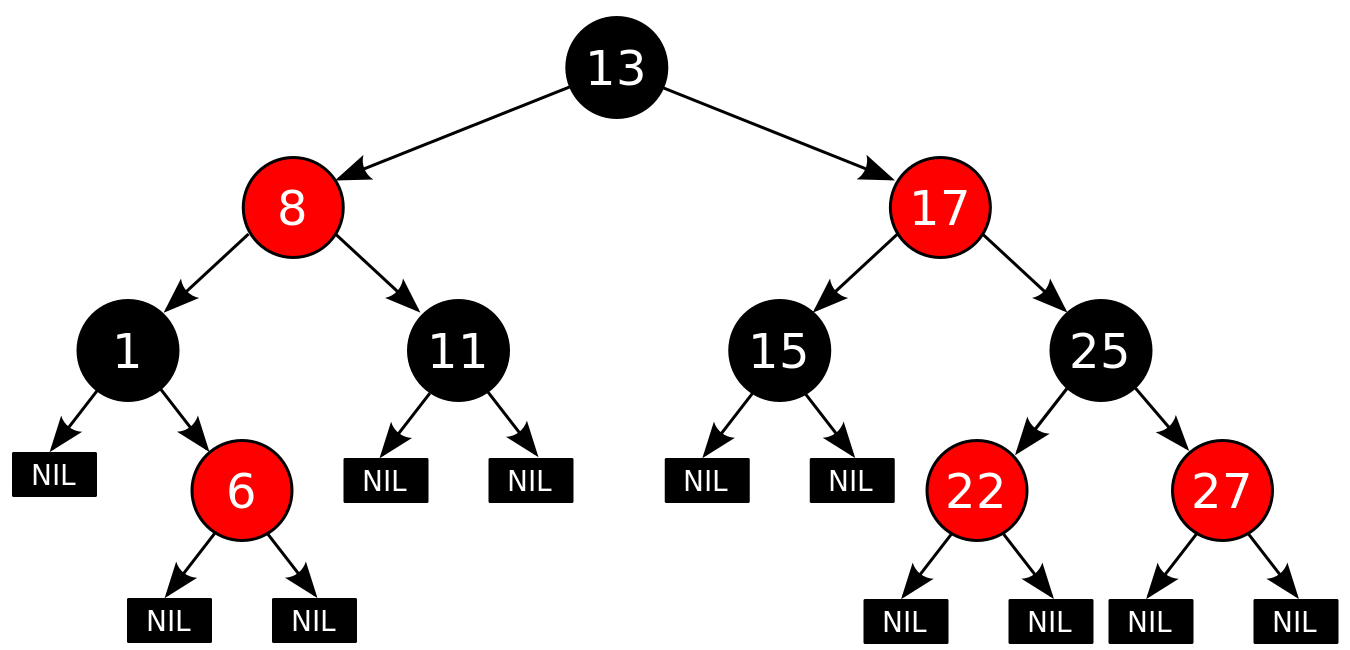
\includegraphics[width=\textwidth]{images/Red-black_tree_example}};

      \tikz[align=left] \node [below=of rbtree,node font=\tiny\itshape] {By Cburnett -- Own work, CC
        BY-SA 3.0\\https://commons.wikimedia.org/w/index.php?curid=1508398};
    \end{column}

    \begin{column}{.5\textwidth}<3->
      \setlength{\bytesize}{0.2cm}
      \setlength{\memwidth}{8\bytesize}
      \setlength{\memheight}{5cm}

      \begin{tikzpicture}[
          word/.style={
            draw=black!50,
            minimum height=\bytesize,
            minimum width=8\bytesize,
            inner sep=0pt
          },
          anchor=south west
        ]

        \node (word) at (0,0) [word,fill=blue!90!black,text=white] {\tiny value};
        \node (next) [word,above=0 of word,fill=red!90!black] {};
        \node (prev) [word,above=0 of next,fill=yellow!90!black] {};
        \node (parent) [word,above=0 of prev,fill=green!90!black] {};
        \node (color) [word,above=0 of parent,fill=black!20!white] {};
        \node [above left=0 and -\bytesize of parent,
          rectangle,
          inner sep=0pt,
          minimum width=\bytesize,
          minimum height=\bytesize,
          draw=black!50,
          fill=none,
          label={90:{\tiny color}}
        ] {};

        \node (wordp) [word,above right=1.1 and .1 of word,fill=blue!90!black,opacity=.3] {};
        \node (nextp) [word,above=0 of wordp,fill=red!90!black,opacity=.3] {};
        \node (prevp) [word,above=0 of nextp,fill=yellow!90!black,opacity=.3] {};
        \node (parentp) [word,above=0 of prevp,fill=green!90!black,opacity=.3] {};
        \node (colorp) [word,above=0 of parentp,fill=black!20!white,opacity=.3] {};

        \node (wordl) [word,below left=1.1 and .1 of word,fill=blue!90!black,opacity=.3] {};
        \node (nextl) [word,above=0 of wordl,fill=red!90!black,opacity=.3] {};
        \node (prevl) [word,above=0 of nextl,fill=yellow!90!black,opacity=.3] {};
        \node (parentl) [word,above=0 of prevl,fill=green!90!black,opacity=.3] {};
        \node (colorl) [word,above=0 of parentl,fill=black!20!white,opacity=.3] {};

        \node (wordr) [word,below right=1.1 and .1 of word,fill=blue!90!black,opacity=.3] {};
        \node (nextr) [word,above=0 of wordr,fill=red!90!black,opacity=.3] {};
        \node (prevr) [word,above=0 of nextr,fill=yellow!90!black,opacity=.3] {};
        \node (parentr) [word,above=0 of prevr,fill=green!90!black,opacity=.3] {};
        \node (colorr) [word,above=0 of parentr,fill=black!20!white,opacity=.3] {};

        \draw[{Circle[length=2pt]}-Stealth,black!80] (parent.east) to [out=0,in=270] node[auto,swap] {\tiny parent} (wordp.south);
        \draw[{Circle[length=2pt]}-Stealth,black!80] (prev.west) to [out=180,in=90] node[auto,swap] {\tiny left} (colorl.north);
        \draw[{Circle[length=2pt]}-Stealth,black!80] (next.east) to [out=0,in=90] node[auto,swap] {\tiny right} (colorr.north);

      \end{tikzpicture}
    \end{column}
  \end{columns}
\end{frame}

\begin{frame}{Hands-on}
  \begin{itemize}
  \item C++ $\rightarrow$ Containers
  \item Inspect, build and run \code{containers.cpp}, also using \code{perf}
  \item Extend it to manage an \code{std::list}
  \item Compare the performance obtained with the two containers
  \end{itemize}
\end{frame}
